\chapter{Reading a station model}\label{p3-ch:station}

\textit{This chapter answers Map Q12.}

\section{Why a station model?}

About 10\,000 weather stations around the world measure as many as 18 quantities at each observation: temperature, dew point, pressure, wind, cloud, weather, and more. To show all that on one map the World Meteorological Organization (WMO) fixed a compact way of drawing an observation, the \textbf{station model}. Every number and symbol has a fixed position around a small circle that marks the station. Once you know the positions, a map becomes a table you can read at a glance.

\section{The anatomy of a station model}

\newcommand{\modelpic}[2]{\begin{tikzpicture}[x=0.052cm,y=-0.052cm,line cap=round]\input{generated/#1}#2\end{tikzpicture}}
\newcommand{\leader}[4]{\draw[gray,thin] (#1,#2) -- (#3,#4);}

\begin{figure}[ht]
\centering
\modelpic{model_anatomy.tex}{
  \leader{-24}{-24}{-70}{-62}\node[anchor=east,font=\scriptsize,align=right] at (-72,-62) {\textbf{wind:} the staff points to where\\ the wind comes \emph{from};\\ barbs give the speed};
  \leader{-26}{-13}{-100}{-22}\node[anchor=east,font=\scriptsize,align=right] at (-102,-22) {\textbf{air temperature} ($^\circ$F)};
  \leader{22}{-14}{70}{-60}\node[anchor=west,font=\scriptsize,align=left] at (72,-62) {\textbf{pressure}, in tenths of a hPa,\\ with the leading 9 or 10 omitted};
  \leader{36}{4}{110}{-6}\node[anchor=west,font=\scriptsize,align=left] at (112,-6) {\textbf{pressure change} in the\\ last 3 hours, and its pattern};
  \leader{-26}{8}{-100}{18}\node[anchor=east,font=\scriptsize,align=right] at (-102,18) {\textbf{present weather}\\ (here: continuous rain)};
  \leader{-26}{24}{-84}{54}\node[anchor=east,font=\scriptsize,align=right] at (-86,56) {\textbf{dew point} ($^\circ$F)};
  \leader{5}{7}{58}{62}\node[anchor=west,font=\scriptsize,align=left] at (60,64) {\textbf{sky cover:} how much of the\\ sky is covered by cloud};
}
\caption{A station model with every field labelled. This example reads: temperature 45\,\degF, dew point 38\,\degF, pressure 1014.7\,hPa, rising by 2.8\,hPa in the last three hours, three-quarters of the sky covered, continuous rain, and a wind of 20\,knots from the north-west.}\label{p3-fig:anatomy}
\end{figure}

\begin{table}[ht]
\centering
\caption{Where each quantity sits around the circle.}
\begin{tabular}{@{}ll@{}}
\toprule
\textbf{Position} & \textbf{What it shows}\\
\midrule
Top left & air temperature, in \degF\ here\\
Bottom left & dew-point temperature\\
Top right & pressure: three digits (tenths of a hectopascal)\\
Right, below the pressure & pressure change over the last 3 hours (with a symbol for its pattern)\\
Left of the circle & present weather symbol\\
The circle itself & sky cover (how much is filled)\\
A line from the circle & wind: the staff points \textbf{from} where the wind blows, barbs give the speed\\
\bottomrule
\end{tabular}
\end{table}

\section{Decoding the pressure}

Only three digits are plotted, in tenths of a hectopascal, and the leading digits are left off. Sea-level pressure almost always lies between about 950 and 1050\,hPa, so the missing digits can be restored without doubt.

\begin{keybox}[The pressure rule]
\begin{enumerate}[label=\textbf{\arabic*.},itemsep=2pt]
\item Put a decimal point before the last digit: $117\to11.7$.
\item If the three-digit number is \textbf{less than 500}, put \textbf{10} in front: $11.7\to1011.7$\,hPa.
\item If it is \textbf{500 or more}, put \textbf{9} in front: $998\to99.8\to999.8$\,hPa.
\end{enumerate}
\end{keybox}

\begin{table}[ht]
\centering
\caption{Examples of the pressure rule (the first four are the models of Question~12).}
\begin{tabular}{ccccl}
\toprule
\textbf{Code} & \textbf{Decimal point} & \textbf{$<500$ or $\ge500$?} & \textbf{Prefix} & \textbf{Pressure}\\
\midrule
024 & 02.4 & $<500$ & 10 & \textbf{1002.4 hPa}\\
998 & 99.8 & $\ge500$ & 9 & \textbf{999.8 hPa}\\
117 & 11.7 & $<500$ & 10 & \textbf{1011.7 hPa}\\
997 & 99.7 & $\ge500$ & 9 & \textbf{999.7 hPa}\\
147 & 14.7 & $<500$ & 10 & 1014.7 hPa\\
\bottomrule
\end{tabular}
\end{table}

\section{Temperature and dew point}

Both are in degrees Fahrenheit here. To convert to Celsius, subtract 32 and multiply by 5/9:
\begin{equation}
T(\degC)=\tfrac{5}{9}\,[T(\degF)-32].\label{p3-eq:ftoc}
\end{equation}
\begin{where}
T(\degC),\ T(\degF) & the same temperature in Celsius and in Fahrenheit & \degF\ from the station model\\
\end{where}
So 37\,\degF\ is 2.8\,\degC, 63\,\degF\ is 17.2\,\degC, and 21\,\degF\ is $-6.1$\,\degC.

The \textbf{dew point is the water-vapour measure of Chapter~\ref{p3-ch:dew}}, and the gap between the two, $T-T_d$, tells you how close the air is to saturation. A gap of 3\,\degF\ means nearly saturated air (fog, rain or thick cloud likely); a gap of 20\,\degF\ means dry air. You can turn the pair into a relative humidity with the formula $\mathrm{RH}=100\,e_s(T_d)/e_s(T)$.

\section{Sky cover}

The circle is filled in proportion to the cloud cover. Here it is in tenths. The shading grows clockwise from the top, as in Figure~\ref{p3-fig:sky}.

\begin{figure}[ht]
\centering
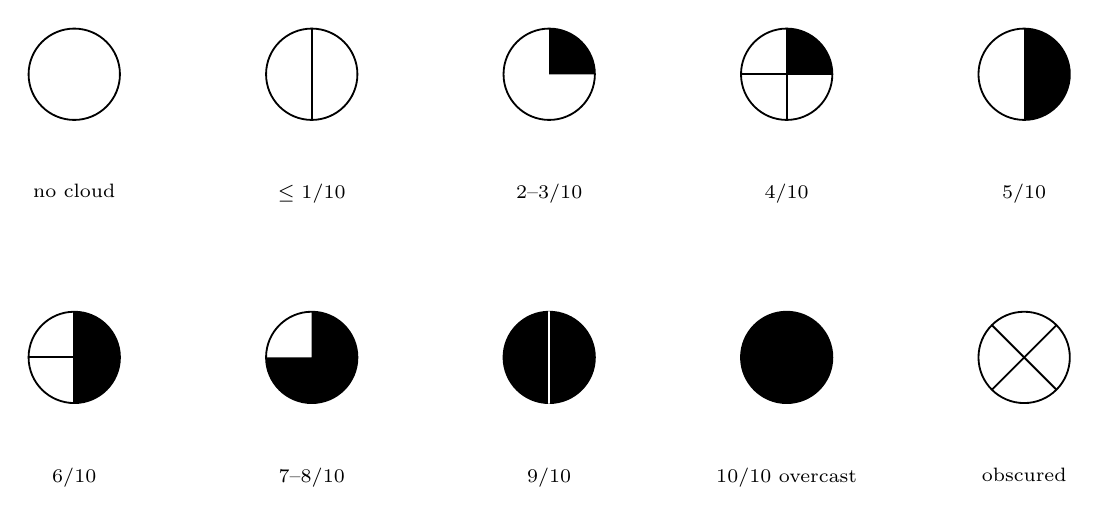
\begin{tikzpicture}[x=0.058cm,y=-0.058cm,line cap=round]\draw[black,line width=0.66pt,fill=white] (24.0,20.0) circle (10.0);
\node[anchor=north,inner sep=0pt,font=\fontsize{7.5}{7.5}\selectfont,text=black] at (24.0,44.0) {no cloud};
\draw[black,line width=0.66pt,fill=white] (76.0,20.0) circle (10.0);
\draw[black,line width=0.66pt] (76.0,10.0) -- (76.0,30.0);
\node[anchor=north,inner sep=0pt,font=\fontsize{7.5}{7.5}\selectfont,text=black] at (76.0,44.0) {$\le 1/10$};
\draw[black,line width=0.66pt,fill=white] (128.0,20.0) circle (10.0);
\fill[black] (128.0,20.0) -- (128.0,10.0) -- (129.3,10.1) -- (130.6,10.3) -- (131.8,10.8) -- (133.0,11.3) -- (134.1,12.1) -- (135.1,12.9) -- (135.9,13.9) -- (136.7,15.0) -- (137.2,16.2) -- (137.7,17.4) -- (137.9,18.7) -- (138.0,20.0) -- cycle;
\node[anchor=north,inner sep=0pt,font=\fontsize{7.5}{7.5}\selectfont,text=black] at (128.0,44.0) {2--3/10};
\draw[black,line width=0.66pt,fill=white] (180.0,20.0) circle (10.0);
\fill[black] (180.0,20.0) -- (180.0,10.0) -- (181.3,10.1) -- (182.6,10.3) -- (183.8,10.8) -- (185.0,11.3) -- (186.1,12.1) -- (187.1,12.9) -- (187.9,13.9) -- (188.7,15.0) -- (189.2,16.2) -- (189.7,17.4) -- (189.9,18.7) -- (190.0,20.0) -- cycle;
\draw[black,line width=0.66pt] (170.0,20.0) -- (190.0,20.0);
\draw[black,line width=0.66pt] (180.0,10.0) -- (180.0,30.0);
\node[anchor=north,inner sep=0pt,font=\fontsize{7.5}{7.5}\selectfont,text=black] at (180.0,44.0) {4/10};
\draw[black,line width=0.66pt,fill=white] (232.0,20.0) circle (10.0);
\fill[black] (232.0,20.0) -- (232.0,10.0) -- (233.3,10.1) -- (234.6,10.3) -- (235.8,10.8) -- (237.0,11.3) -- (238.1,12.1) -- (239.1,12.9) -- (239.9,13.9) -- (240.7,15.0) -- (241.2,16.2) -- (241.7,17.4) -- (241.9,18.7) -- (242.0,20.0) -- (241.9,21.3) -- (241.7,22.6) -- (241.2,23.8) -- (240.7,25.0) -- (239.9,26.1) -- (239.1,27.1) -- (238.1,27.9) -- (237.0,28.7) -- (235.8,29.2) -- (234.6,29.7) -- (233.3,29.9) -- (232.0,30.0) -- cycle;
\node[anchor=north,inner sep=0pt,font=\fontsize{7.5}{7.5}\selectfont,text=black] at (232.0,44.0) {5/10};
\draw[black,line width=0.66pt,fill=white] (24.0,82.0) circle (10.0);
\fill[black] (24.0,82.0) -- (24.0,72.0) -- (25.3,72.1) -- (26.6,72.3) -- (27.8,72.8) -- (29.0,73.3) -- (30.1,74.1) -- (31.1,74.9) -- (31.9,75.9) -- (32.7,77.0) -- (33.2,78.2) -- (33.7,79.4) -- (33.9,80.7) -- (34.0,82.0) -- (33.9,83.3) -- (33.7,84.6) -- (33.2,85.8) -- (32.7,87.0) -- (31.9,88.1) -- (31.1,89.1) -- (30.1,89.9) -- (29.0,90.7) -- (27.8,91.2) -- (26.6,91.7) -- (25.3,91.9) -- (24.0,92.0) -- cycle;
\draw[black,line width=0.66pt] (14.0,82.0) -- (34.0,82.0);
\draw[black,line width=0.66pt] (24.0,72.0) -- (24.0,92.0);
\node[anchor=north,inner sep=0pt,font=\fontsize{7.5}{7.5}\selectfont,text=black] at (24.0,106.0) {6/10};
\draw[black,line width=0.66pt,fill=white] (76.0,82.0) circle (10.0);
\fill[black] (76.0,82.0) -- (76.0,72.0) -- (77.3,72.1) -- (78.6,72.3) -- (79.8,72.8) -- (81.0,73.3) -- (82.1,74.1) -- (83.1,74.9) -- (83.9,75.9) -- (84.7,77.0) -- (85.2,78.2) -- (85.7,79.4) -- (85.9,80.7) -- (86.0,82.0) -- (85.9,83.3) -- (85.7,84.6) -- (85.2,85.8) -- (84.7,87.0) -- (83.9,88.1) -- (83.1,89.1) -- (82.1,89.9) -- (81.0,90.7) -- (79.8,91.2) -- (78.6,91.7) -- (77.3,91.9) -- (76.0,92.0) -- (74.7,91.9) -- (73.4,91.7) -- (72.2,91.2) -- (71.0,90.7) -- (69.9,89.9) -- (68.9,89.1) -- (68.1,88.1) -- (67.3,87.0) -- (66.8,85.8) -- (66.3,84.6) -- (66.1,83.3) -- (66.0,82.0) -- cycle;
\node[anchor=north,inner sep=0pt,font=\fontsize{7.5}{7.5}\selectfont,text=black] at (76.0,106.0) {7--8/10};
\draw[black,line width=0.66pt,fill=white] (128.0,82.0) circle (10.0);
\fill[black] (128.0,82.0) circle (10.0);
\draw[white,line width=0.66pt] (128.0,72.0) -- (128.0,92.0);
\node[anchor=north,inner sep=0pt,font=\fontsize{7.5}{7.5}\selectfont,text=black] at (128.0,106.0) {9/10};
\draw[black,line width=0.66pt,fill=white] (180.0,82.0) circle (10.0);
\fill[black] (180.0,82.0) circle (10.0);
\node[anchor=north,inner sep=0pt,font=\fontsize{7.5}{7.5}\selectfont,text=black] at (180.0,106.0) {10/10 overcast};
\draw[black,line width=0.66pt,fill=white] (232.0,82.0) circle (10.0);
\draw[black,line width=0.66pt] (225.0,75.0) -- (239.0,89.0);
\draw[black,line width=0.66pt] (239.0,75.0) -- (225.0,89.0);
\node[anchor=north,inner sep=0pt,font=\fontsize{7.5}{7.5}\selectfont,text=black] at (232.0,106.0) {obscured};
\end{tikzpicture}
\caption{The sky-cover symbols: from clear (empty) through half (right half filled) to overcast (filled), and an obscured sky (a cross). The ``9/10'' symbol is filled with a vertical gap: overcast with small openings.}\label{p3-fig:sky}
\end{figure}

\section{Wind: the barbs}

The wind is drawn as a straight line, the \textbf{staff}, that starts at the circle and points \textbf{towards the direction the wind comes from}, as a weather vane does. At the free end are short lines, the \textbf{barbs}, that tell you the speed in knots.

\begin{itemize}
\item a \textbf{half barb}: 5 knots;
\item a \textbf{full barb}: 10 knots;
\item a \textbf{pennant} (a filled triangle): 50 knots;
\item no barb but a staff: 1 to 2 knots; a circle round the station and no staff: calm.
\end{itemize}

\begin{figure}[ht]
\centering
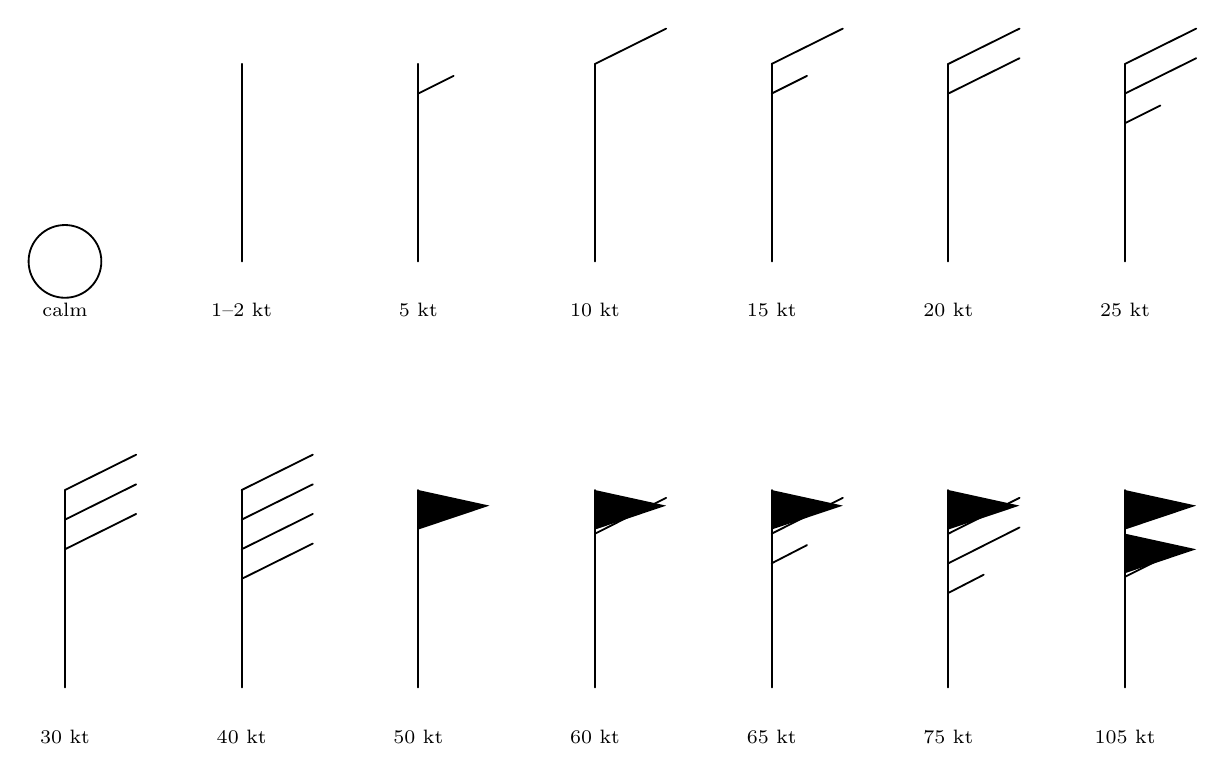
\begin{tikzpicture}[x=0.066cm,y=-0.066cm,line cap=round]\draw[black,line width=0.66pt] (24.0,52.0) circle (7.0);
\node[anchor=north,inner sep=0pt,font=\fontsize{7.5}{7.5}\selectfont,text=black] at (24.0,60.0) {calm};
\draw[black,line width=0.66pt] (58.0,52.0) -- (58.0,14.0);
\node[anchor=north,inner sep=0pt,font=\fontsize{7.5}{7.5}\selectfont,text=black] at (58.0,60.0) {1--2 kt};
\draw[black,line width=0.66pt] (92.0,52.0) -- (92.0,14.0);
\draw[black,line width=0.66pt] (92.0,19.7) -- (98.8,16.3);
\node[anchor=north,inner sep=0pt,font=\fontsize{7.5}{7.5}\selectfont,text=black] at (92.0,60.0) {5 kt};
\draw[black,line width=0.66pt] (126.0,52.0) -- (126.0,14.0);
\draw[black,line width=0.66pt] (126.0,14.0) -- (139.7,7.2);
\node[anchor=north,inner sep=0pt,font=\fontsize{7.5}{7.5}\selectfont,text=black] at (126.0,60.0) {10 kt};
\draw[black,line width=0.66pt] (160.0,52.0) -- (160.0,14.0);
\draw[black,line width=0.66pt] (160.0,14.0) -- (173.7,7.2);
\draw[black,line width=0.66pt] (160.0,19.7) -- (166.8,16.3);
\node[anchor=north,inner sep=0pt,font=\fontsize{7.5}{7.5}\selectfont,text=black] at (160.0,60.0) {15 kt};
\draw[black,line width=0.66pt] (194.0,52.0) -- (194.0,14.0);
\draw[black,line width=0.66pt] (194.0,14.0) -- (207.7,7.2);
\draw[black,line width=0.66pt] (194.0,19.7) -- (207.7,12.9);
\node[anchor=north,inner sep=0pt,font=\fontsize{7.5}{7.5}\selectfont,text=black] at (194.0,60.0) {20 kt};
\draw[black,line width=0.66pt] (228.0,52.0) -- (228.0,14.0);
\draw[black,line width=0.66pt] (228.0,14.0) -- (241.7,7.2);
\draw[black,line width=0.66pt] (228.0,19.7) -- (241.7,12.9);
\draw[black,line width=0.66pt] (228.0,25.4) -- (234.8,22.0);
\node[anchor=north,inner sep=0pt,font=\fontsize{7.5}{7.5}\selectfont,text=black] at (228.0,60.0) {25 kt};
\draw[black,line width=0.66pt] (24.0,134.0) -- (24.0,96.0);
\draw[black,line width=0.66pt] (24.0,96.0) -- (37.7,89.2);
\draw[black,line width=0.66pt] (24.0,101.7) -- (37.7,94.9);
\draw[black,line width=0.66pt] (24.0,107.4) -- (37.7,100.6);
\node[anchor=north,inner sep=0pt,font=\fontsize{7.5}{7.5}\selectfont,text=black] at (24.0,142.0) {30 kt};
\draw[black,line width=0.66pt] (58.0,134.0) -- (58.0,96.0);
\draw[black,line width=0.66pt] (58.0,96.0) -- (71.7,89.2);
\draw[black,line width=0.66pt] (58.0,101.7) -- (71.7,94.9);
\draw[black,line width=0.66pt] (58.0,107.4) -- (71.7,100.6);
\draw[black,line width=0.66pt] (58.0,113.1) -- (71.7,106.3);
\node[anchor=north,inner sep=0pt,font=\fontsize{7.5}{7.5}\selectfont,text=black] at (58.0,142.0) {40 kt};
\draw[black,line width=0.66pt] (92.0,134.0) -- (92.0,96.0);
\fill[black] (92.0,96.0) -- (105.7,99.0) -- (92.0,103.6) -- cycle;
\node[anchor=north,inner sep=0pt,font=\fontsize{7.5}{7.5}\selectfont,text=black] at (92.0,142.0) {50 kt};
\draw[black,line width=0.66pt] (126.0,134.0) -- (126.0,96.0);
\fill[black] (126.0,96.0) -- (139.7,99.0) -- (126.0,103.6) -- cycle;
\draw[black,line width=0.66pt] (126.0,104.4) -- (139.7,97.5);
\node[anchor=north,inner sep=0pt,font=\fontsize{7.5}{7.5}\selectfont,text=black] at (126.0,142.0) {60 kt};
\draw[black,line width=0.66pt] (160.0,134.0) -- (160.0,96.0);
\fill[black] (160.0,96.0) -- (173.7,99.0) -- (160.0,103.6) -- cycle;
\draw[black,line width=0.66pt] (160.0,104.4) -- (173.7,97.5);
\draw[black,line width=0.66pt] (160.0,110.1) -- (166.8,106.6);
\node[anchor=north,inner sep=0pt,font=\fontsize{7.5}{7.5}\selectfont,text=black] at (160.0,142.0) {65 kt};
\draw[black,line width=0.66pt] (194.0,134.0) -- (194.0,96.0);
\fill[black] (194.0,96.0) -- (207.7,99.0) -- (194.0,103.6) -- cycle;
\draw[black,line width=0.66pt] (194.0,104.4) -- (207.7,97.5);
\draw[black,line width=0.66pt] (194.0,110.1) -- (207.7,103.2);
\draw[black,line width=0.66pt] (194.0,115.8) -- (200.8,112.3);
\node[anchor=north,inner sep=0pt,font=\fontsize{7.5}{7.5}\selectfont,text=black] at (194.0,142.0) {75 kt};
\draw[black,line width=0.66pt] (228.0,134.0) -- (228.0,96.0);
\fill[black] (228.0,96.0) -- (241.7,99.0) -- (228.0,103.6) -- cycle;
\fill[black] (228.0,104.4) -- (241.7,107.4) -- (228.0,112.0) -- cycle;
\draw[black,line width=0.66pt] (228.0,112.7) -- (234.8,109.3);
\node[anchor=north,inner sep=0pt,font=\fontsize{7.5}{7.5}\selectfont,text=black] at (228.0,142.0) {105 kt};
\end{tikzpicture}
\caption{Wind barbs for the Northern Hemisphere, drawn with the staff pointing up (a north wind) and the barbs on the right. Add the barbs: 10 + 10 + 5 = 25 knots.}
\end{figure}

\textbf{To read a barb.}
\begin{enumerate}[label=\textbf{Step \arabic*.},leftmargin=*,itemsep=3pt]
\item Find the staff and follow it from the circle to its free end. The wind comes \emph{from} that direction: a staff pointing to the lower left is a wind from the south-west.
\item Count the barbs at the free end: pennants (50), full barbs (10), half barbs (5). Add them.
\item Convert if you wish: 1\,knot $=0.514\ \ms$, so 25\,knots $=12.9\ \ms$.
\end{enumerate}

\begin{askbox}
\textbf{The staff points where the wind comes from, but the air is moving the other way. Which way do I draw a streamline?}\\
Away from the barbs, i.e.\ in the direction \emph{opposite} to the staff. A staff pointing to the south-west means the air is heading north-east. Keep that in mind in Chapter~\ref{p3-ch:stream}.
\end{askbox}

\section{Present weather and pressure tendency}

\begin{figure}[ht]
\centering
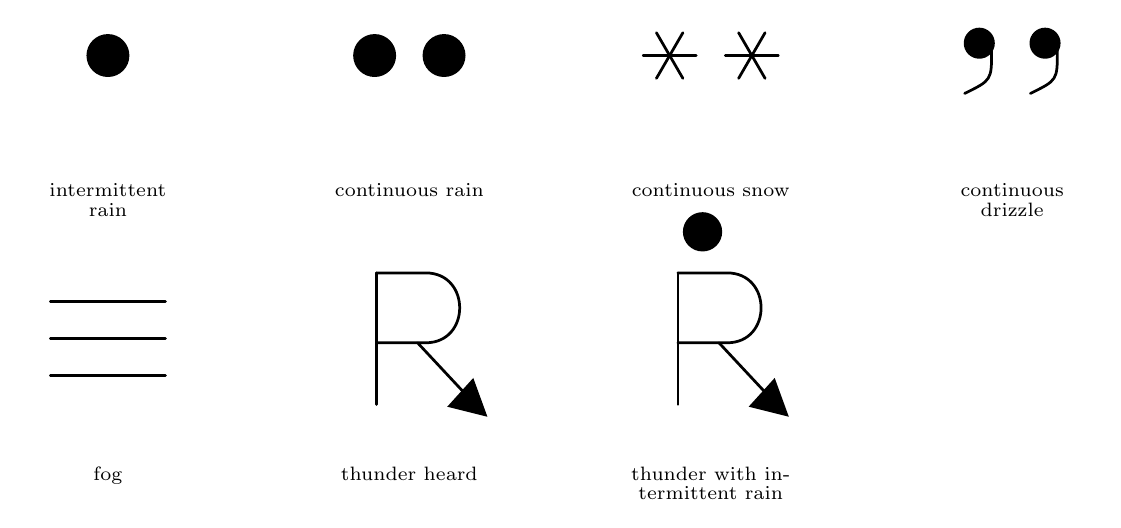
\begin{tikzpicture}[x=0.058cm,y=-0.058cm,line cap=round]\fill[black] (34.0,26.0) circle (4.7);
\node[anchor=north,inner sep=0pt,font=\fontsize{7.0}{7.0}\selectfont,text=black,align=center,text width=58pt] at (34.0,54.0) {intermittent rain};
\fill[black] (92.4,26.0) circle (4.7);
\fill[black] (107.6,26.0) circle (4.7);
\node[anchor=north,inner sep=0pt,font=\fontsize{7.0}{7.0}\selectfont,text=black,align=center,text width=58pt] at (100.0,54.0) {continuous rain};
\draw[black,line width=0.99pt] (151.2,26.0) -- (162.8,26.0);
\draw[black,line width=0.99pt] (154.1,21.0) -- (159.9,31.0);
\draw[black,line width=0.99pt] (159.9,21.0) -- (154.1,31.0);
\draw[black,line width=0.99pt] (169.2,26.0) -- (180.8,26.0);
\draw[black,line width=0.99pt] (172.1,21.0) -- (177.9,31.0);
\draw[black,line width=0.99pt] (177.9,21.0) -- (172.1,31.0);
\node[anchor=north,inner sep=0pt,font=\fontsize{7.0}{7.0}\selectfont,text=black,align=center,text width=58pt] at (166.0,54.0) {continuous snow};
\fill[black] (224.8,23.3) circle (3.4);
\draw[black,line width=0.99pt] (227.5,24.9) .. controls (227.5,31.4) .. (221.6,34.3);
\fill[black] (239.2,23.3) circle (3.4);
\draw[black,line width=0.99pt] (241.9,24.9) .. controls (241.9,31.4) .. (236.0,34.3);
\node[anchor=north,inner sep=0pt,font=\fontsize{7.0}{7.0}\selectfont,text=black,align=center,text width=58pt] at (232.0,54.0) {continuous drizzle};
\draw[black,line width=0.99pt] (21.4,79.9) -- (46.6,79.9);
\draw[black,line width=0.99pt] (21.4,88.0) -- (46.6,88.0);
\draw[black,line width=0.99pt] (21.4,96.1) -- (46.6,96.1);
\node[anchor=north,inner sep=0pt,font=\fontsize{7.0}{7.0}\selectfont,text=black,align=center,text width=58pt] at (34.0,116.0) {fog};
\draw[black,line width=0.99pt] (92.8,73.6) -- (92.8,102.4);
\draw[black,line width=0.99pt] (92.8,73.6) -- (103.6,73.6) .. controls (113.5,73.6) and (113.5,88.9) .. (103.6,88.9) -- (92.8,88.9);
\draw[black,line width=0.99pt] (101.8,88.9) -- (114.4,102.4);
\fill[black] (117.1,105.1) -- (108.3,102.9) -- (114.0,96.6) -- cycle;
\node[anchor=north,inner sep=0pt,font=\fontsize{7.0}{7.0}\selectfont,text=black,align=center,text width=58pt] at (100.0,116.0) {thunder heard};
\draw[black,line width=0.99pt] (158.8,73.6) -- (158.8,102.4);
\draw[black,line width=0.99pt] (158.8,73.6) -- (169.6,73.6) .. controls (179.5,73.6) and (179.5,88.9) .. (169.6,88.9) -- (158.8,88.9);
\draw[black,line width=0.99pt] (167.8,88.9) -- (180.4,102.4);
\fill[black] (183.1,105.1) -- (174.3,102.9) -- (180.0,96.6) -- cycle;
\fill[black] (164.2,64.6) circle (4.3);
\node[anchor=north,inner sep=0pt,font=\fontsize{7.0}{7.0}\selectfont,text=black,align=center,text width=58pt] at (166.0,116.0) {thunder with intermittent rain};
\end{tikzpicture}
\caption{The present-weather symbols used here.}
\end{figure}

\begin{figure}[ht]
\centering
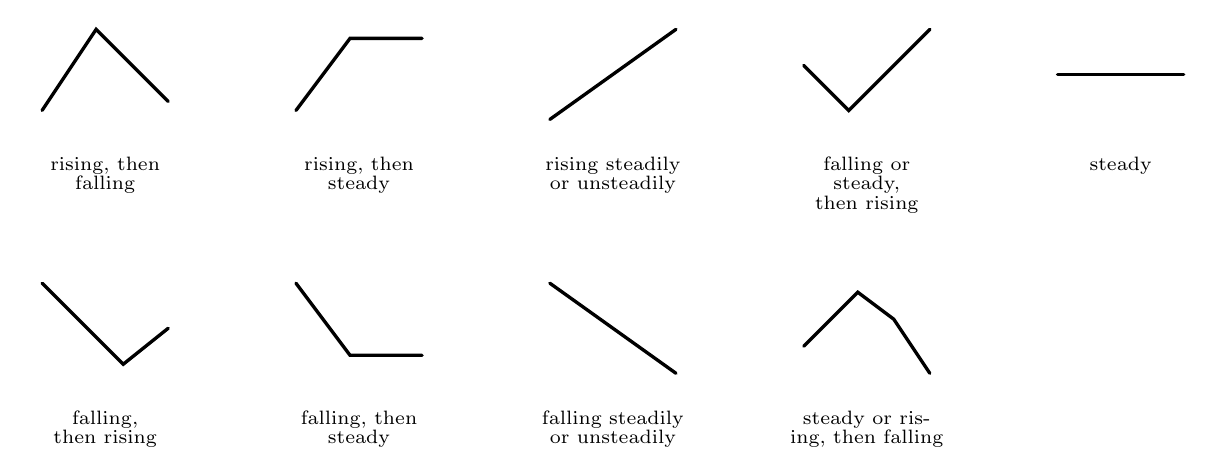
\begin{tikzpicture}[x=0.052cm,y=-0.052cm,line cap=round]\draw[black,line width=1.21pt] (12.6,32.8) -- (25.8,13.0) -- (32.4,19.6) -- (43.4,30.6);
\node[anchor=north,inner sep=0pt,font=\fontsize{7.0}{7.0}\selectfont,text=black,align=center,text width=56pt] at (28.0,44.0) {rising, then falling};
\draw[black,line width=1.21pt] (74.6,32.8) -- (87.8,15.2) -- (105.4,15.2);
\node[anchor=north,inner sep=0pt,font=\fontsize{7.0}{7.0}\selectfont,text=black,align=center,text width=56pt] at (90.0,44.0) {rising, then steady};
\draw[black,line width=1.21pt] (136.6,35.0) -- (167.4,13.0);
\node[anchor=north,inner sep=0pt,font=\fontsize{7.0}{7.0}\selectfont,text=black,align=center,text width=56pt] at (152.0,44.0) {rising steadily or unsteadily};
\draw[black,line width=1.21pt] (198.6,21.8) -- (209.6,32.8) -- (229.4,13.0);
\node[anchor=north,inner sep=0pt,font=\fontsize{7.0}{7.0}\selectfont,text=black,align=center,text width=56pt] at (214.0,44.0) {falling or steady, then rising};
\draw[black,line width=1.21pt] (260.6,24.0) -- (291.4,24.0);
\node[anchor=north,inner sep=0pt,font=\fontsize{7.0}{7.0}\selectfont,text=black,align=center,text width=56pt] at (276.0,44.0) {steady};
\draw[black,line width=1.21pt] (12.6,75.0) -- (32.4,94.8) -- (43.4,86.0);
\node[anchor=north,inner sep=0pt,font=\fontsize{7.0}{7.0}\selectfont,text=black,align=center,text width=56pt] at (28.0,106.0) {falling, then rising};
\draw[black,line width=1.21pt] (74.6,75.0) -- (87.8,92.6) -- (105.4,92.6);
\node[anchor=north,inner sep=0pt,font=\fontsize{7.0}{7.0}\selectfont,text=black,align=center,text width=56pt] at (90.0,106.0) {falling, then steady};
\draw[black,line width=1.21pt] (136.6,75.0) -- (167.4,97.0);
\node[anchor=north,inner sep=0pt,font=\fontsize{7.0}{7.0}\selectfont,text=black,align=center,text width=56pt] at (152.0,106.0) {falling steadily or unsteadily};
\draw[black,line width=1.21pt] (198.6,90.4) -- (211.8,77.2) -- (220.6,83.8) -- (229.4,97.0);
\node[anchor=north,inner sep=0pt,font=\fontsize{7.0}{7.0}\selectfont,text=black,align=center,text width=56pt] at (214.0,106.0) {steady or rising, then falling};
\end{tikzpicture}
\caption{The barometric tendency symbols: how the pressure has changed in the last three hours. A line rising to the right means rising pressure, one falling to the right means falling pressure.}
\end{figure}

The number next to the symbol, for example $+17$ or $-11$, is the pressure change in tenths of a hectopascal: $+17$ is a rise of 1.7\,hPa in three hours, $-11$ a fall of 1.1\,hPa. Rapid falls often warn of a storm approaching; rising pressure usually brings improving weather.

\section{Question 12: the four station models}\label{p3-sec:sheetmodels}

\begin{questionbox}
Decode the information from each of the following station models.
\end{questionbox}

\textbf{Method.} For each model work down this list: pressure; temperature; dew point; sky cover; and, where shown, current weather, wind speed, wind direction, pressure change and tendency.

\subsection*{Model 1}
\begin{center}
\modelpic{model_sheet1.tex}{
  \leader{-14}{-14}{-64}{-42}\node[anchor=east,font=\scriptsize,text=gray!50!black] at (-66,-42) {temperature};
  \leader{-14}{22}{-64}{44}\node[anchor=east,font=\scriptsize,text=gray!50!black] at (-66,44) {dew point};
  \leader{14}{-14}{64}{-42}\node[anchor=west,font=\scriptsize,text=gray!50!black] at (66,-42) {pressure};
  \leader{6}{5}{56}{30}\node[anchor=west,font=\scriptsize,text=gray!50!black] at (58,30) {sky: empty circle};
}
\end{center}
\begin{answerbox}[Model 1]\small
\textbf{Pressure:} 024 $\to$ 02.4 $\to$ \textbf{1002.4\,hPa}\\
\textbf{Temperature:} \textbf{37\,\degF}\ (2.8\,\degC)\qquad \textbf{Dew point:} \textbf{21\,\degF}\ ($-6.1$\,\degC)\\
\textbf{Sky cover:} empty circle: \textbf{0\,\%} (clear). No staff, only a ring round the circle: \textbf{calm}. RH $\approx52\,\%$.
\end{answerbox}
\subsection*{Model 2}
\begin{center}
\modelpic{model_sheet2.tex}{
  \leader{-14}{-14}{-64}{-42}\node[anchor=east,font=\scriptsize,text=gray!50!black] at (-66,-42) {temperature};
  \leader{-14}{22}{-64}{44}\node[anchor=east,font=\scriptsize,text=gray!50!black] at (-66,44) {dew point};
  \leader{14}{-14}{64}{-42}\node[anchor=west,font=\scriptsize,text=gray!50!black] at (66,-42) {pressure};
  \leader{-24}{6}{-70}{10}\node[anchor=east,font=\scriptsize,text=gray!50!black] at (-72,10) {present weather};
  \leader{6}{5}{56}{30}\node[anchor=west,font=\scriptsize,text=gray!50!black] at (58,30) {sky: half filled};
}
\end{center}
\begin{answerbox}[Model 2]\small
\textbf{Pressure:} 998 $\to$ 99.8 $\to$ \textbf{999.8\,hPa}\\
\textbf{Temperature:} \textbf{63\,\degF}\ (17.2\,\degC)\qquad \textbf{Dew point:} \textbf{60\,\degF}\ (15.6\,\degC)\\
\textbf{Current weather:} \textbf{thunder with intermittent rain}. Sky half filled (5/10); no staff: calm. RH $\approx90\,\%$.
\end{answerbox}

\subsection*{Model 3}
\begin{center}
\modelpic{model_sheet3.tex}{
  \leader{-14}{-14}{-64}{-42}\node[anchor=east,font=\scriptsize,text=gray!50!black] at (-66,-42) {temperature};
  \leader{-14}{22}{-64}{44}\node[anchor=east,font=\scriptsize,text=gray!50!black] at (-66,44) {dew point};
  \leader{14}{-14}{64}{-42}\node[anchor=west,font=\scriptsize,text=gray!50!black] at (66,-42) {pressure};
  \leader{40}{5}{76}{-4}\node[anchor=west,font=\scriptsize,text=gray!50!black] at (78,-4) {pressure change};
  \leader{-30}{30}{-70}{66}\node[anchor=east,font=\scriptsize,text=gray!50!black] at (-72,66) {wind staff};
}
\end{center}
\begin{answerbox}[Model 3]\small
\textbf{Pressure:} 117 $\to$ 11.7 $\to$ \textbf{1011.7\,hPa}\\
\textbf{Temperature:} \textbf{43\,\degF}\ (6.1\,\degC)\qquad \textbf{Dew point:} \textbf{20\,\degF}\ ($-6.7$\,\degC)\qquad \textbf{Sky cover:} empty circle, \textbf{0\,\%}\\
\textbf{Wind:} staff to the lower left: \textbf{from the south-west}; two full barbs and a half barb: \textbf{25 knots}\\
\textbf{Pressure change:} $+17$: \textbf{$+1.7$\,mb}, \textbf{rising}
\end{answerbox}

\subsection*{Model 4}
\begin{center}
\modelpic{model_sheet4.tex}{
  \leader{-14}{-14}{-64}{-42}\node[anchor=east,font=\scriptsize,text=gray!50!black] at (-66,-42) {temperature};
  \leader{-14}{22}{-64}{44}\node[anchor=east,font=\scriptsize,text=gray!50!black] at (-66,44) {dew point};
  \leader{14}{-14}{64}{-42}\node[anchor=west,font=\scriptsize,text=gray!50!black] at (66,-42) {pressure};
  \leader{40}{5}{76}{-4}\node[anchor=west,font=\scriptsize,text=gray!50!black] at (78,-4) {pressure change};
  \leader{-24}{6}{-70}{10}\node[anchor=east,font=\scriptsize,text=gray!50!black] at (-72,10) {present weather};
}
\end{center}
\begin{answerbox}[Model 4]\small
\textbf{Pressure:} 997 $\to$ 99.7 $\to$ \textbf{999.7\,mb}\\
\textbf{Temperature:} \textbf{27\,\degF}\ ($-2.8$\,\degC)\qquad \textbf{Dew point:} \textbf{20\,\degF}\ ($-6.7$\,\degC)\\
\textbf{Sky cover:} filled circle, \textbf{100\,\%}\qquad \textbf{Current weather:} \textbf{continuous snow}\\
\textbf{Wind:} staff to the upper left: \textbf{from the north-west}, \textbf{25 knots}\\
\textbf{Pressure change:} $-11$: \textbf{$-1.1$\,mb}, \textbf{falling}
\end{answerbox}

\medskip
\begin{table}[ht]
\centering
\caption{All four models decoded.}
\begin{tabular}{lcccc}
\toprule
 & \textbf{Model 1} & \textbf{Model 2} & \textbf{Model 3} & \textbf{Model 4}\\
\midrule
Barometric pressure (mb) & 1002.4 & 999.8 & 1011.7 & 999.7\\
Temperature (\degF) & 37 & 63 & 43 & 27\\
Dew point (\degF) & \textbf{21} & 60 & 20 & 20\\
Sky coverage (\%) & 0 & 50 & 0 & 100\\
Current weather & --- & thunder, interm.\ rain & --- & continuous snow\\
Wind speed (knots) & calm & calm & 25 & 25\\
Wind direction (from) & --- & --- & south-west & north-west\\
Pressure change in 3\,h (mb) & --- & --- & $+1.7$ & $-1.1$\\
Tendency & --- & --- & rising & falling\\
\bottomrule
\end{tabular}
\end{table}

\section{What the models tell you}

Putting the numbers together gives each station a story.
\begin{itemize}
\item \textbf{Model 1:} cold, dry (the dew point is 16\,\degF\ below the temperature), clear and calm: a cold, high-pressure night.
\item \textbf{Model 2:} warm and very humid (the dew point only 3\,\degF\ below the temperature), with thunder and rain: unstable, thundery air.
\item \textbf{Model 3:} clear and windy with rising pressure: air moving away from a low towards a high, after a front has passed.
\item \textbf{Model 4:} overcast, snowing, 27\,\degF, wind 25 knots and falling pressure: a depression is arriving or overhead.
\end{itemize}

\section{Try it yourself: Practice Set~\thechapter}

Decode each of the three models in Figure~\ref{p3-fig:practiceG} (pressure, temperature and dew point in \degF\ and \degC, relative humidity, sky cover, weather, wind speed and direction, pressure change and tendency), then check against the answers below.

\begin{figure}[ht]
\centering
\begin{minipage}{0.32\textwidth}\centering \modelpic{model_practice1.tex}{\node[font=\small\bfseries] at (0,70) {G1};}\end{minipage}
\begin{minipage}{0.32\textwidth}\centering \modelpic{model_practice2.tex}{\node[font=\small\bfseries] at (0,70) {G2};}\end{minipage}
\begin{minipage}{0.32\textwidth}\centering \modelpic{model_practice3.tex}{\node[font=\small\bfseries] at (0,70) {G3};}\end{minipage}
\caption{Three station models to decode.}\label{p3-fig:practiceG}
\end{figure}

\begin{answerbox}[Answers to Practice Set~\thechapter]
\begin{enumerate}[label=\textbf{\thechapter.\arabic*},leftmargin=*,itemsep=3pt]
\item \textbf{150} $\to$ 15.0 $\to$ \textbf{1015.0\,hPa}. $T=72$\,\degF\ (22.2\,\degC), $T_d=65$\,\degF\ (18.3\,\degC), RH $\approx79\,\%$. Sky: 2--3/10 (about 25\,\%). Wind: staff pointing straight down: \textbf{from the south}, one full barb and a half barb: \textbf{15\,knots}. Tendency: $+21$ $\to$ up 2.1\,hPa, rising then steady. No weather symbol: fair, warm and humid.
\item \textbf{975} ($\ge500$) $\to$ 97.5 $\to$ \textbf{997.5\,hPa}. $T=48$\,\degF\ (8.9\,\degC), $T_d=47$\,\degF\ (8.3\,\degC); RH $\approx96\,\%$. Overcast (100\,\%). Continuous rain. Wind from the \textbf{north-east}, three full barbs and a half barb: \textbf{35\,knots}. Pressure $-32$: down 3.2\,hPa, falling steadily.
\item \textbf{084} ($<500$) $\to$ 08.4 $\to$ \textbf{1008.4\,hPa}. $T=5$\,\degF\ ($-15$\,\degC), $T_d=3$\,\degF; RH $\approx91\,\%$. Sky: 6/10. Continuous drizzle. Wind from the \textbf{west}, one full barb: \textbf{10\,knots}. Pressure $-4$: down 0.4\,hPa, rising then falling.
\end{enumerate}
\end{answerbox}

\section{Station models in Python}

These functions compute the equations of this chapter, and the book's tests check them against its answers.

\lstinputlisting{../../atmosphere_atlas/practical3_guide/generated/fn_fahrenheit_to_celsius.py}
\lstinputlisting{../../atmosphere_atlas/practical3_guide/generated/fn_decode_pressure.py}
\lstinputlisting{../../atmosphere_atlas/practical3_guide/generated/fn_knots_to_ms.py}

\verb|decode_pressure(247)| returns 1024.7 and \verb|decode_pressure(987)| returns 998.7.
